%%%%%%%%%%%%%%%%%%%%%%%%%%%%%%%%%%%%%%%%%%%%%%%%%%%%%%%%%%%%%%%%%%%%%%%%%%%%%%%%
\documentclass[letterpaper, 10 pt, conference]{ieeeconf}  % Comment this line out
                                                          % if you need a4paper
%\documentclass[a4paper, 10pt, conference]{ieeeconf}      % Use this line for a4
                                                          % paper

\usepackage{hyperref} % Chris - hyperlink all the things
\usepackage{todonotes} % Chris - nice todo notes!
\usepackage{listings} % Chris - include some code formatting stuff
\usepackage{textcomp} % Chris - fixes warnings due to gensymb below
\usepackage{gensymb} % Chris - so we can have \degrees

\IEEEoverridecommandlockouts                              % This command is only
                                                          % needed if you want to
                                                          % use the \thanks command
\overrideIEEEmargins
% See the \addtolength command later in the file to balance the column lengths
% on the last page of the document

\setlength{\marginparwidth}{1.5cm} % Chris added this to correct display of in margin todo's

% The following packages can be found on http:\\www.ctan.org
\usepackage{graphicx} % for pdf, bitmapped graphics files
%\usepackage{epsfig} % for postscript graphics files
%\usepackage{mathptmx} % assumes new font selection scheme installed
%\usepackage{times} % assumes new font selection scheme installed
%\usepackage{amsmath} % assumes amsmath package installed
%\usepackage{amssymb}  % assumes amsmath package installed

\title{\LARGE \bf
Validation of IMU-Based Hand Pose Tracking System \\ WPI RBE 580 Final Project
}

%\author{ \parbox{3 in}{\centering Huibert Kwakernaak*
%         \thanks{*Use the $\backslash$thanks command to put information here}\\
%         Faculty of Electrical Engineering, Mathematics and Computer Science\\
%         University of Twente\\
%         7500 AE Enschede, The Netherlands\\
%         {\tt\small h.kwakernaak@autsubmit.com}}
%         \hspace*{ 0.5 in}
%         \parbox{3 in}{ \centering Pradeep Misra**
%         \thanks{**The footnote marks may be inserted manually}\\
%        Department of Electrical Engineering \\
%         Wright State University\\
%         Dayton, OH 45435, USA\\
%         {\tt\small pmisra@cs.wright.edu}}
%}

\author{Christopher Bove, Rahul Krishnan, Shreyash Shantha Kumar, Luis Lasa}
% \author{Huibert Kwakernaak$^{1}$ and Pradeep Misra$^{2}$% <-this % stops a space
% \thanks{*This work was not supported by any organization}% <-this % stops a space
% \thanks{$^{1}$H. Kwakernaak is with Faculty of Electrical Engineering, Mathematics and Computer Science,
%         University of Twente, 7500 AE Enschede, The Netherlands
%         {\tt\small h.kwakernaak at papercept.net}}%
% \thanks{$^{2}$P. Misra is with the Department of Electrical Engineering, Wright State University,
%         Dayton, OH 45435, USA
%         {\tt\small p.misra at ieee.org}}%
% }


\begin{document}

\maketitle
\thispagestyle{empty}
\pagestyle{empty}


%%%%%%%%%%%%%%%%%%%%%%%%%%%%% ABSTRACT %%%%%%%%%%%%%%%%%%%%%%%%%%%%%%%%%
\begin{abstract}
In stroke victim rehabilitation or research concerning Parkinson's disease, it is often useful to capture data of the patients' hand movements. Typical hand and finger tracking hardware is expensive, and while IMU-based approaches are cheaper, their characteristics and accuracy are less well-known across a range of circumstances. In this project, a portable hand pose tracking unit was validated through comparison to results from a motion capture system. A test bed was created to robustly test finger bending motions, and the IMU's were interfaced with an Arduino Mega to provide synchronized data recording with an OptiTrack motion capture system. Results indicated the IMU-based system had typically small joint angle errors of less than 0.4\degree\ in static tests, up to 2\degree\ of error in prolonged finger bending, up to 10\degree\ of error during shaking motions, 0.5\degree\ of error with ferrous material interference, and 1\degree\ of error with magnetic interference. These results indicate the IMU-based system is fairly accurate in normal circumstances even with environmental disturbances, but may be less suitable in circumstances where the hand shakes very violently.
\end{abstract}

%%%%%%%%%%%%%%%%%%%%%%%%%%%%% INTRODUCTION %%%%%%%%%%%%%%%%%%%%%%%%%%%%%%%%%
\section{INTRODUCTION}
Quantification of patient rehabilitation after disease or injury can be very useful in objectively evaluating the effectiveness and patient recovery time of different methods and treatments. For patients with Parkinson's Disease or recovering stroke victims, tracking the hand and finger movements would be useful as they attempted to regain fine motor skills. While there are many systems that can produce accurate data, such as visual motion capture, many of them remain prohibitively expensive for small clinics. There are often lower-cost alternatives, but these offer a trade-off, usually forgoing accuracy or compromising performance under certain conditions. 

The goal of this project was to validate an IMU-based hand pose tracking system that could be implemented for rehabilitation monitoring of stroke victims or patients with Parkinson’s Disease. This effort was developed in Spring 2016 by an RBE 501 project team and WPI's AIM Laboratory. The end result was four absolute orientation IMU's affixed to a cotton glove that could determine the joint angles of the wearer's finger in MATLAB. The team demonstrated sufficient ability to determine finger link orientation, validating the idea that low-cost IMU's could be used for estimation of hand and finger posture.

While it appeared the system achieved about five degrees of link angle accuracy compared to motion capture (mocap) results, testing was not exhaustive. It was not known for how long the system maintained those characteristics. In addition, the IMU's relied on compass data to obtain an orientation estimate, so it was possible that in environments with varying ferrous elements, magnetic fields, or excessive EMF noise, the sensors could exhibit significant reduction in accuracy. It was suggested that more sophisticated and robust testing could illuminate answers to some of those questions.

With this in mind, associates of WPI AIM Laboratory set off to create a more reliable way to robustly test the system. A precisely machined two link mechanism housed IMU’s on each link to track both links' orientation. Retro-reflective markers were placed on the links to enable a mocap system to gather truth data during testing, as shown in \autoref{fig:fingerLink}. This project comes into play by conducting those tests and evaluating the error of the IMU's, change in error over time, and error changes in different situations and circumstances, such as various movement patterns and in the presence of magnetic interference.

\begin{figure}[thpb]
	\centering
	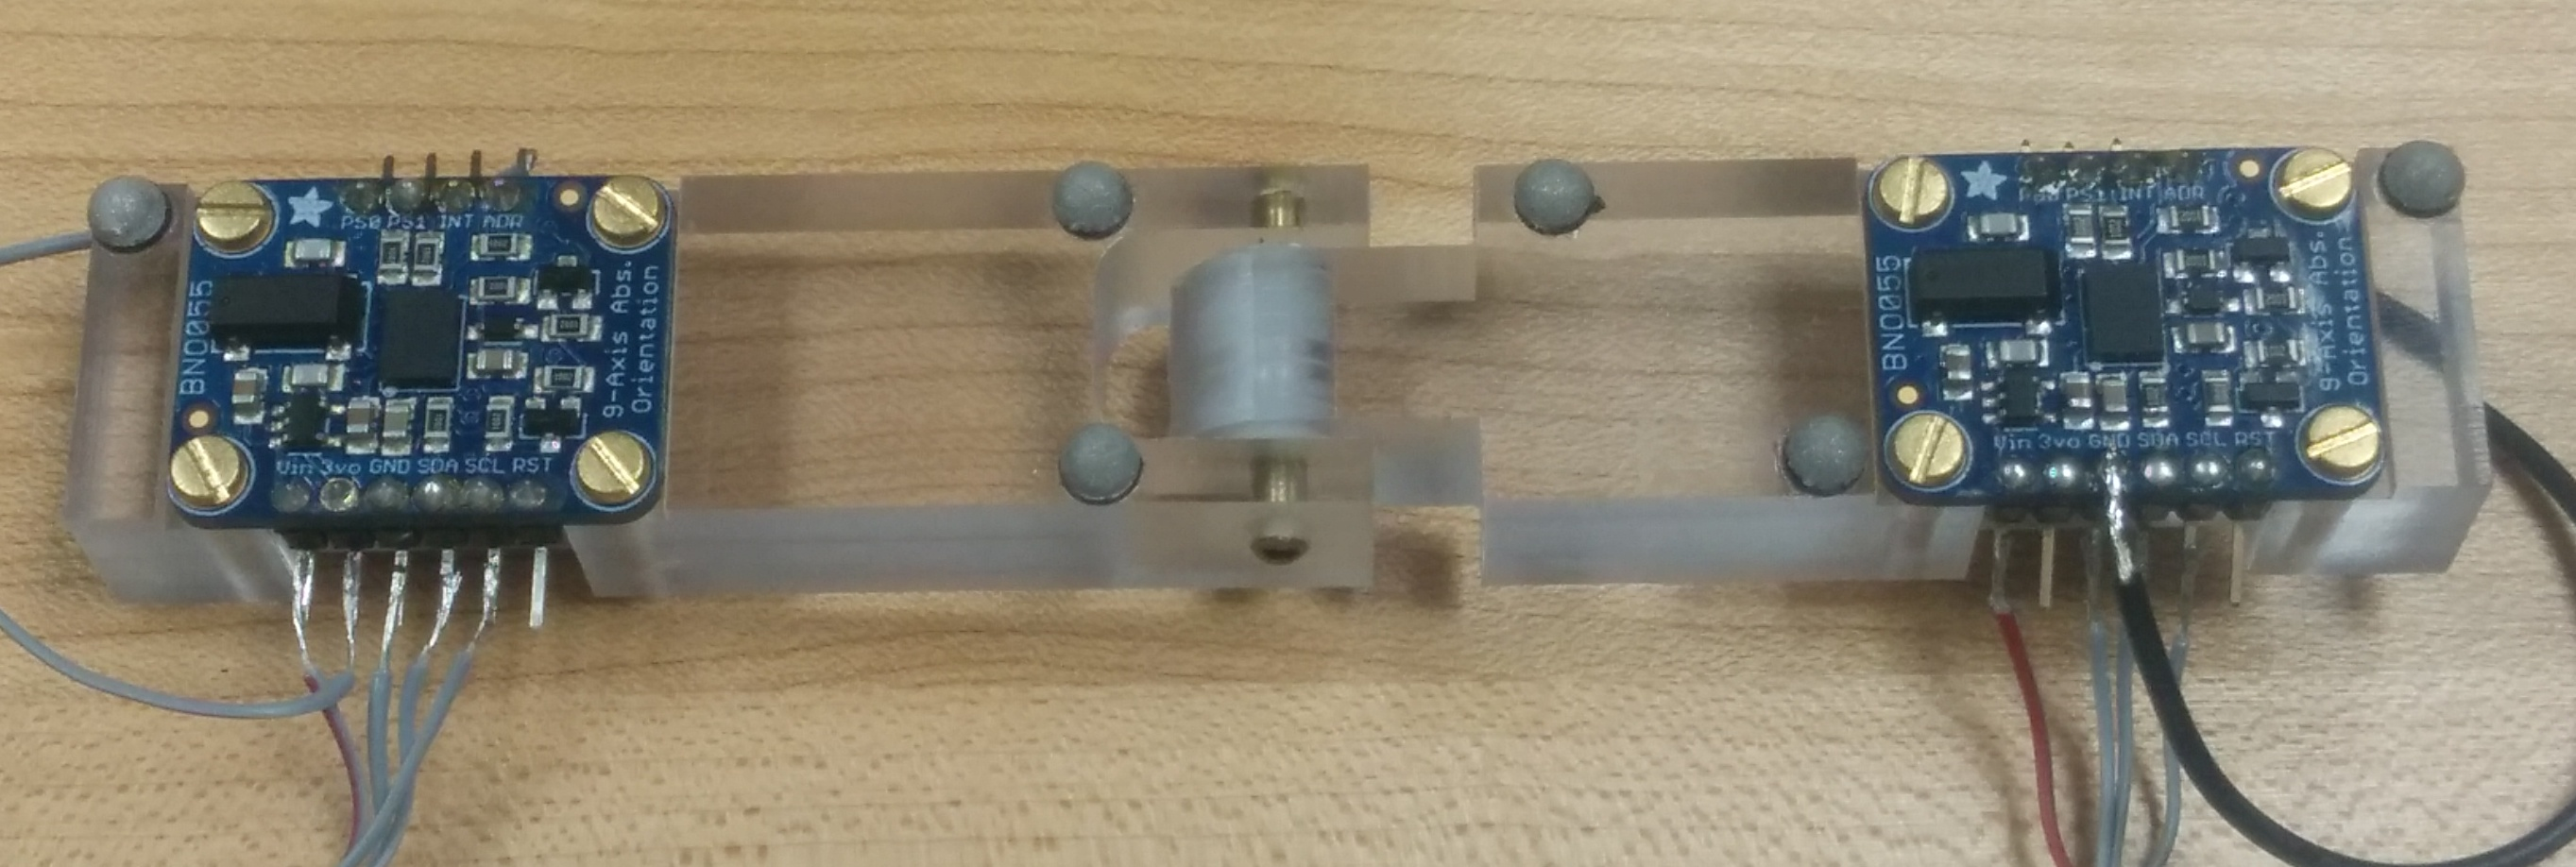
\includegraphics[width = 3in]{finger_link.jpg}
    \caption{Photograph of the acrylic finger link system with attached IMU's and retro-reflective marker spheres for tracking by motion capture system. }
    \label{fig:fingerLink}
\end{figure}

%%%%%%%%%%%%%%%%%%%%%%%%%%%%% BACKGROUND %%%%%%%%%%%%%%%%%%%%%%%%%%%%%%%%%
\section{BACKGROUND}
Sensors are often used in the biomedical field to track movement of the body after disease or injury. Some are incorporated into entire robotic exoskeletons aimed at rehabilitation purposes, while others are used for data monitoring to be used in future research or to determine timing for medical interventions. Patients with Parkinson’s Disease or stroke victims can benefit from these techniques.

Patients with Parkinson’s Disease experience most of their tremors while in a state of rest, and those tremors usually oscillate at a frequency between 4-6Hz \cite{Perumal}. Accelerometers, force sensors, gyroscopes and magnetometers can be used as both to diagnose and monitor the disease \cite{Perumal}, as these provide mechanisms for examining changes in orientation and linear acceleration.

Another useful application of sensor technology is involved in drug release. Patients with Parkinson’s often find their motor capabilities change rapidly, and in order to ensure the highest quality of life, medication must be administered accordingly. This is difficult for doctors, who are often unable to continuously monitor their patients. Sensors designated to react to the intensity of their tremors are used to distribute the appropriate levels of medication \cite{Patel}. In one experiment, a portable three axis accelerometer was attached to the shoulder of the patient, measuring their movement and severity of tremors \cite{Patel}.

Stroke patients are also monitored to see how much damage occurred during the event to their bodies. One study discussed experimentally determining the difference between the “healthy” arm and the arm affected by a stroke. These experiments were conducted using one RF-receiver placed on the wrist and tracking it as the patient completed 3 designated tasks \cite{Sokal}.
\cite{Zhou} examines different types of sensors used in various biomedical applications, and \autoref{table:trackingSystems} shows relative rankings for a variety of sensor technologies according to their research.

\begin{table}[h]
	\scriptsize
	\caption{Tracking Systems Comparison}
	\label{table:trackingSystems}
	\begin{center}
    \renewcommand{\arraystretch}{1.5}
	\begin{tabular}{|p{1.0cm}|p{1cm}|p{0.6cm}|p{1.4cm}|p{0.6cm}|p{1.45cm}|}
	\hline
	\textbf{Systems} & \textbf{Accuracy} & \textbf{Size} & \textbf{Computation} & \textbf{Cost} & \textbf{Drawbacks} \\ \hline
	Inertial & High & Small & Efficient & Low & Drifts \\ \hline
    Magnetic & Med. & Small & Efficient & Low & Ferromagnetic materials \\ \hline
    Ultrasound & Med. & Med. & Efficient & Low & Occlusion \\ \hline
    Glove & High & Med. & Efficient & Med. & Partial Posture \\ \hline
    Marker & High & Med. & Inefficient & Med. & Occlusion \\ \hline 
    Robot & High & Large & Inefficient & High & Limited Motion \\ \hline
	\end{tabular}
	\end{center}
\end{table}

Inertial sensors are non-visual tracking systems that measure acceleration (linear or angular) or other passive forces felt by a body. These devices are typically small, lightweight and compact. However, they are highly susceptible to drift over time and require re-calibration often \cite{Zhou}. Optical tracking systems, on the other hand, are visual tracking systems and require a direct line of sight to the targeted markers. This limitation is a significant drawback if the movement being tracked is complex or rotates away from the camera \cite{Zhou}.

In a project conducted by WPI students in the Spring 2016 RBE 501 class, the team created a finger tracking system using IMU’s.  They attached four IMU's to a glove, one IMU on each link of the finger and one on the back of the hand. This system allowed them to visualize the orientation of each link of a finger and determine where the links intersected at the joint.
Unfortunately, as previously discussed, the data presented in their paper was not extensive.  Because IMU’s are known to drift over time, more thorough and long-term tests are needed to better determine their performance in different positions, situations, and configurations.

%%%%%%%%%%%%%%%%%%%%%%%%%%%%% METHODS %%%%%%%%%%%%%%%%%%%%%%%%%%%%%%%%%
\section{METHODS}

\subsection{Mechanical Hardware}
A testbed was created to evaluate the performance of the system during consistent and repeatable motion. This manifested itself in two mechanisms: one for actuation of the finger link and another for movement of the system as a whole. The finger was actuated through a PWM controlled HS-322HD Hitec servo motor, controlled from an Arduino. The system was moved by hand, but could easily be mounted onto a robotic arm to allow more controlled testing.

For the purpose of coupling the two-link system with the servo motor, a mechanical fastener was 3D printed. SOLIDWORKS was used for the design of the coupling mechanism. As shown in \autoref{fig:couplingCad}, it consisted of two parts: a base where both system and servo were attached, and a clip that grabbed the upper link of the system and the servo horn. The Arduino was be programmed to perform finger-bending motion by changing the PWM control signals to the servo. As shown in \autoref{fig:couplingPhts}, as the servo horn rotated, the upper link turned as well.

\begin{figure}[thpb]
	\centering
	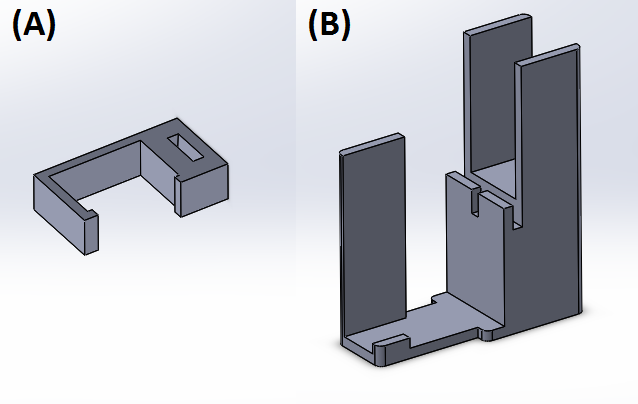
\includegraphics[width = 3in]{coupling_cads.png}
    \caption{(A) Coupling Clip to hold servo horn to movable link. (B) Base fastening the servo and the base link.}
    \label{fig:couplingCad}
\end{figure}

\begin{figure}[thpb]
	\centering
	\includegraphics[width = 3in]{coupling_photos.png}
    \caption{(A) Coupled system on a straight position. (B) Servo actuating the system.}
    \label{fig:couplingPhts}
\end{figure}

\subsection{Electrical Hardware}
The electrical system consisted of two IMUs (Adafruit-packaged BNO055 Bosch sensor on a break out board) interfaced with an Arduino Mega. Since the IMU's were operating on the same I2C bus, one of them needed its address pin pulled high so that it self-assigned a different address to prevent communication problems on the I2C bus. A second Arduino, an Arduino Uno, was interfaced with a Hitech HS-322HD servo motor to control the servo position. A PC communicated with the Arduino Mega via USB serial interface. This PC used Putty to log the serial data streamed from the Arduino. \autoref{fig:wiringDiagram} shows the breadboard view of the two sensors connected to the Arduino Mega. Connection of the servo to the Uno was trivial with the input signal of the servo going to a PWM-compatible pin and the power and ground of the servo connected to Vin and GND on the Arduino respectively.

\begin{figure}[thpb]
	\centering
	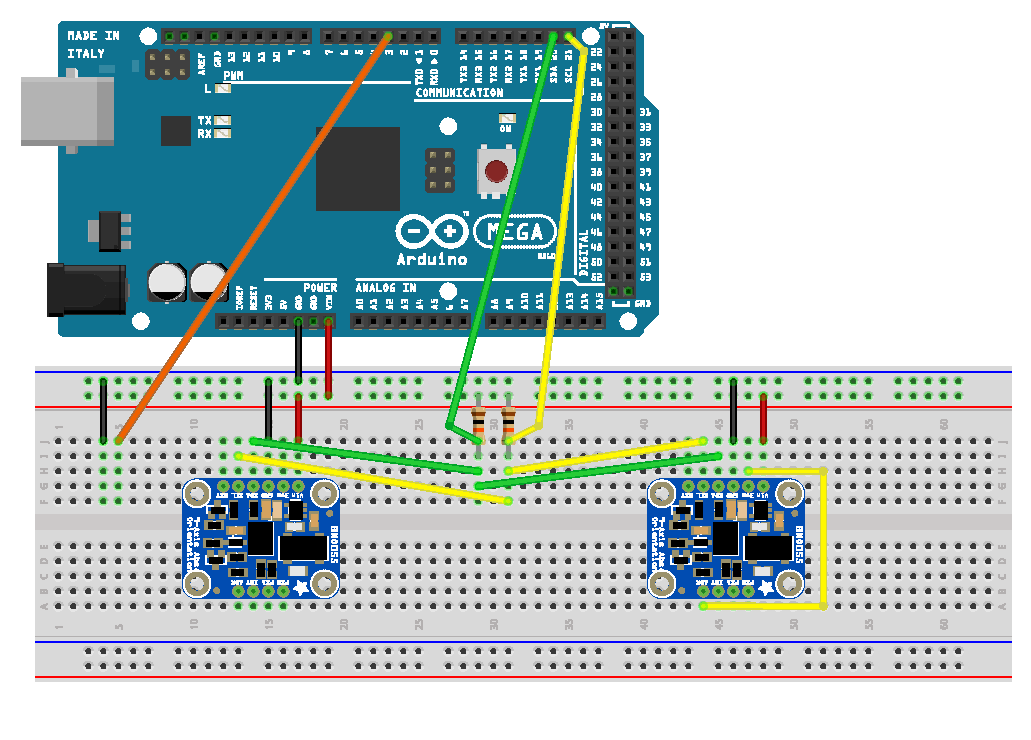
\includegraphics[width = 3in]{Arduino_schematic_bb.pdf}
    \caption{Breadboard wiring view of the Arduino and Adafruit-manufactured BNO055 sensor breakout boards. The unconnected wires at J4 and J5 represent the connections made to the shutter event lines from the mocap system.}
    \label{fig:wiringDiagram}
\end{figure}

\subsection{Motion Capture}
Team members were introduced to the OptiTrack hardware and software suite at AIM Lab. The mocap setup consisted of six \href{http://optitrack.com/products/flex-13/}{OptiTrack Flex 13} cameras capable of recording at up to 120FPS connected to a laptop over USB 2.0. Motive, OptiTrack's proprietary software, was used on the laptop to connect to the cameras, calibrate the system, and record data. The cameras, situated on tripods, were stationed around a small work table, and the system was calibrated through standard ``wanding'' procedures available in Motive, where a line of markers is moved in front of each camera to fully cover the work area and view of the cameras. Afterwards, a new project was created and the markers on the two-link test-bed system were registered in the Motive software suite. This allowed the centroid of each rigid body to be tracked in the system. Data export control was setup so that a CSV file of all 3D data would be created during takes, which included quaternion orientation of each rigid body as well as the positions of all registered markers. In addition, the synchronization settings were modified to provide a shutter output event as a rise on a 3.3V Digital Output line.\footnote{The Arduino digital logic gates enable at 3.0 Volts.} This clocked the Arduino and mocap systems together to ensure minimal latency between mocap and IMU data. \autoref{fig:experimentalSetup} shows the mocap system in the experimental setup.

\begin{figure}[thpb]
	\centering
	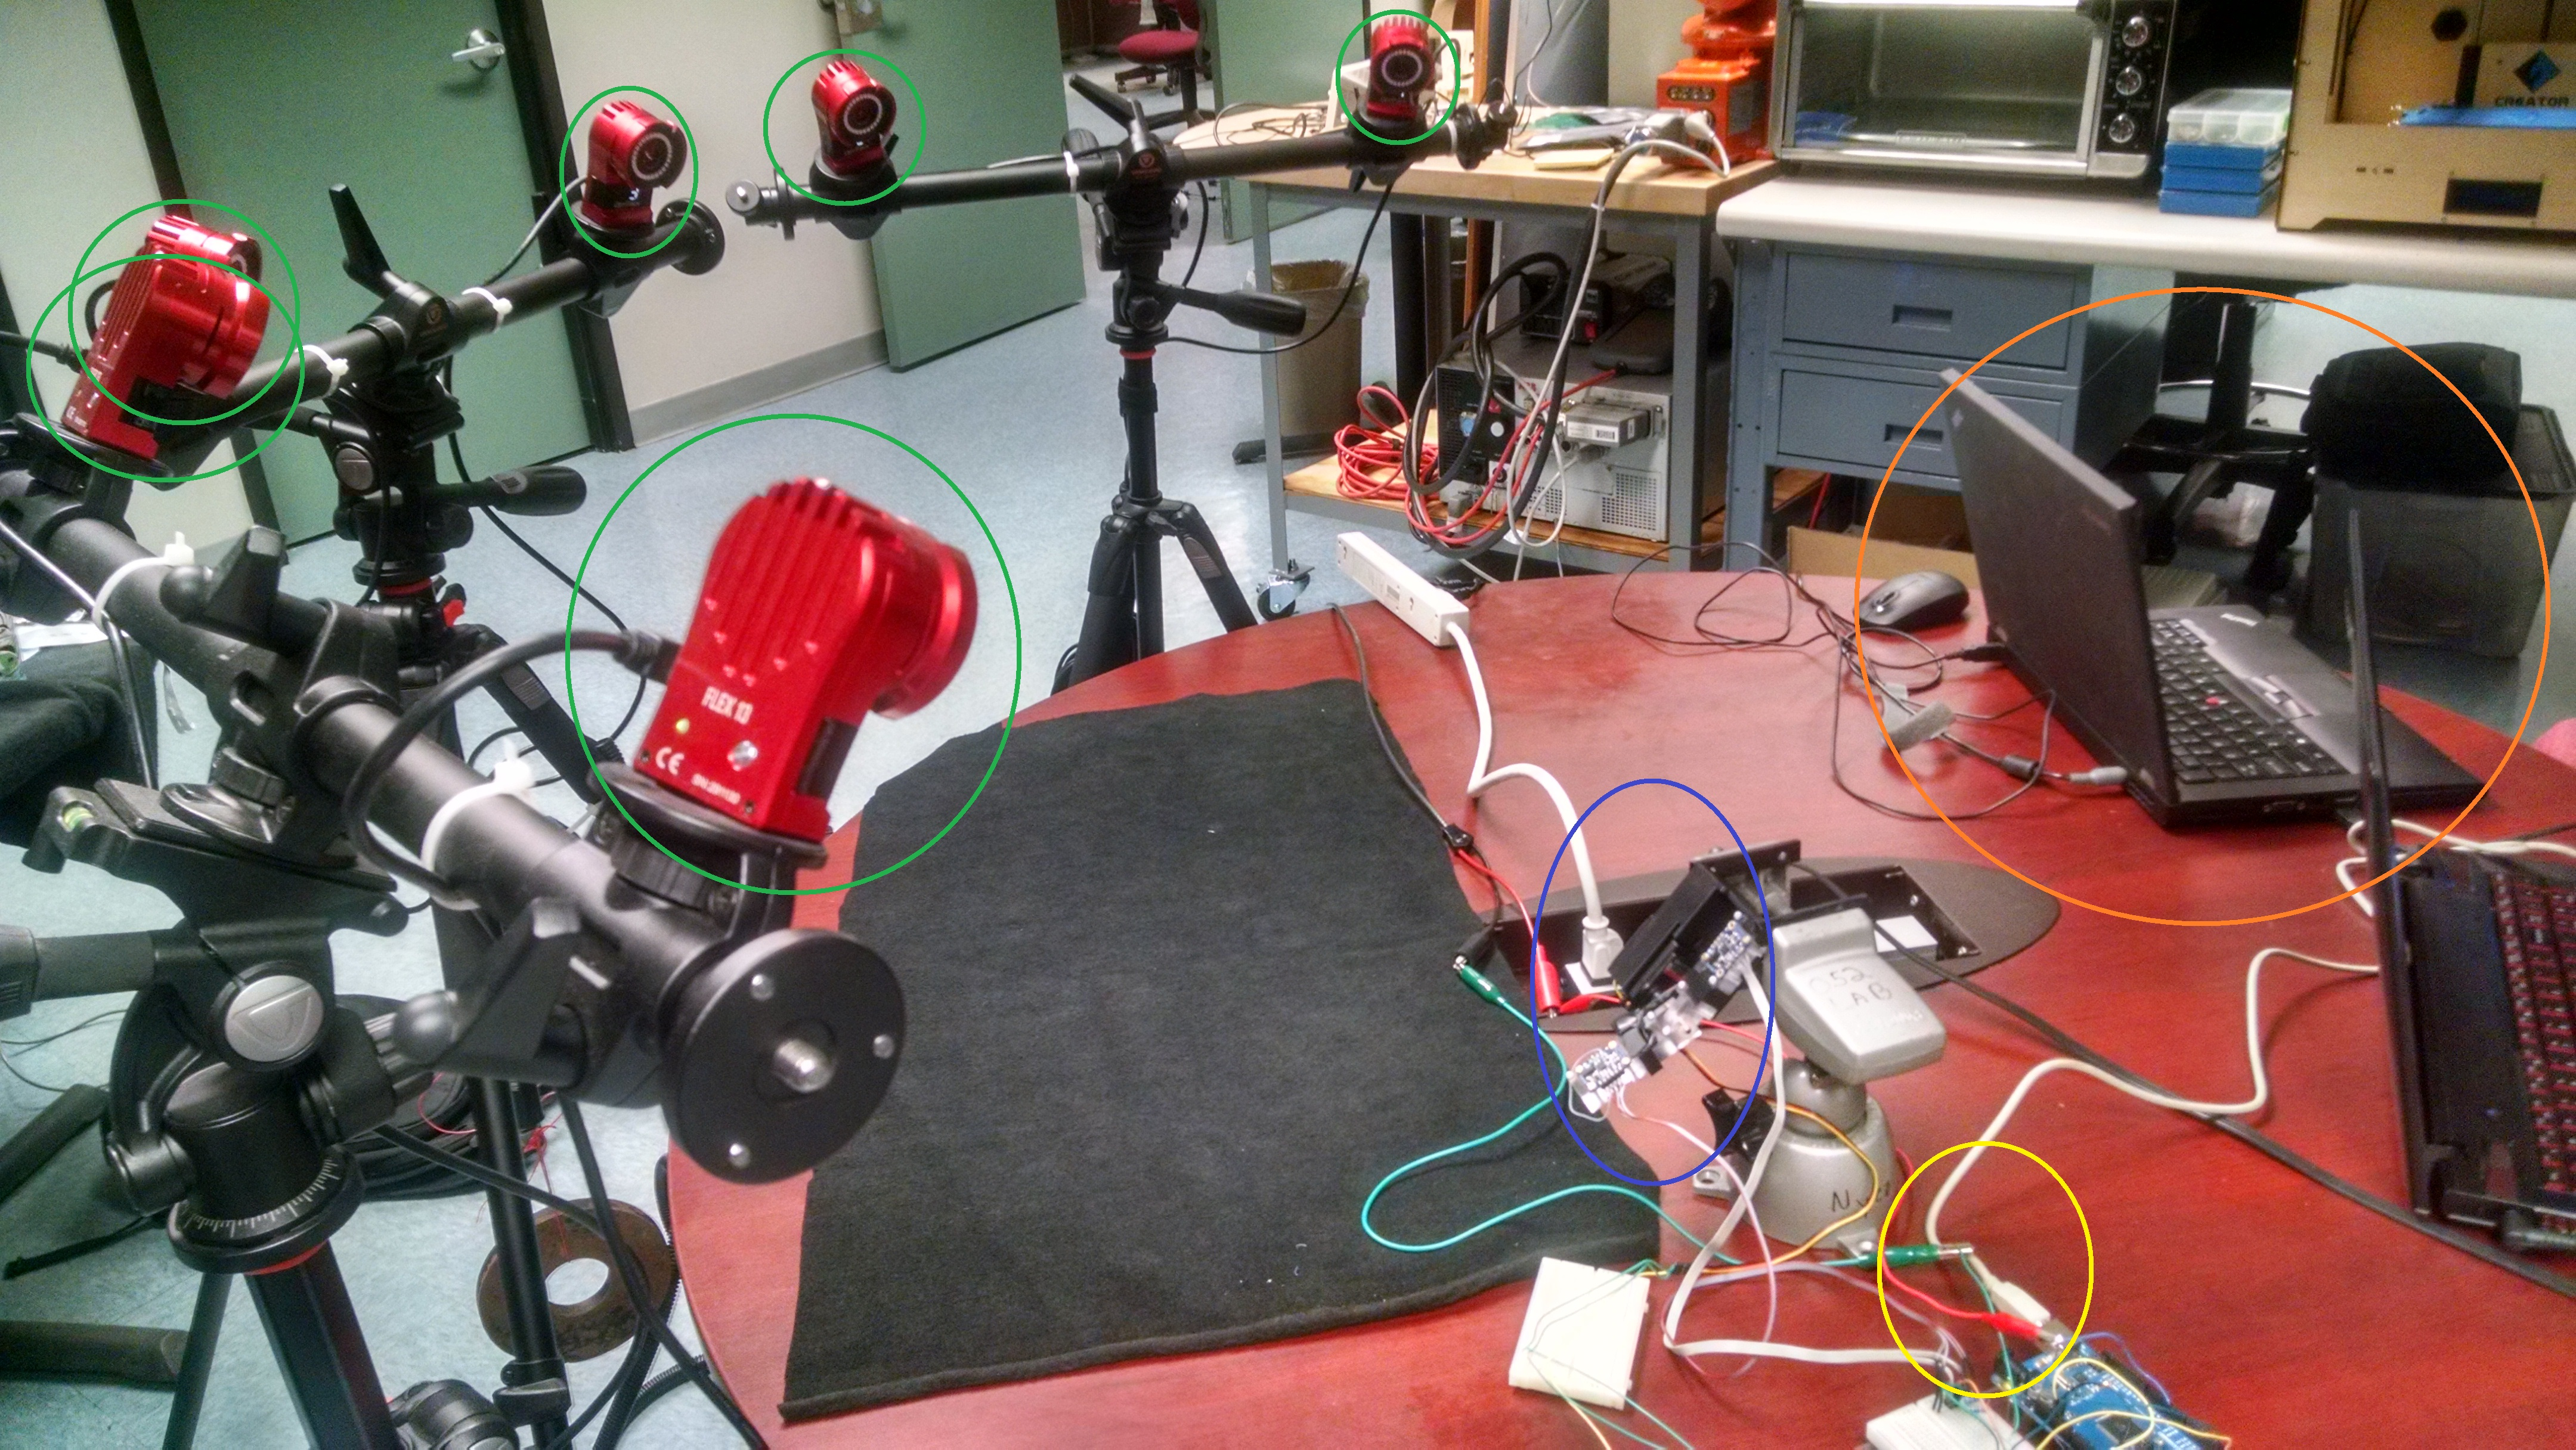
\includegraphics[width = 3in]{experimental_setup.jpg}
    \caption{Experimental setup of the motion capture system and finger link at test. In green are the motion capture cameras, in blue is the system at test, in orange is the digital shutter event line connected to the Arduino Mega, and in orange is the computer connected to motion capture. A second computer was connected to the Ardunio Mega and Arduino Uno (not pictured).}
    \label{fig:experimentalSetup}
\end{figure}

\subsection{Arduino Software}
The code from last year's project was acquired and loaded into a \href{https://github.com/ChrisBove/HandPoseTracking/}{GitHub repository}. The previous team utilized an Arduino Yun, which succeeded the Arduino Uno. Our team was supplied an Arduino Mega, so the code was quickly refactored to compile on the Mega. In addition, the previous team used an I2C MUX to redirect communications to the desired IMU, so modifications were made to the code, using the two distinct IMU addresses 0x28 and 0x29 that supported by the Adafruit BNO055 IMU's. This was fairly straightforward, but electrical problems on the Channel A chip caused some delays. The solder joint on the Channel A pin that pulled the address select to ground was intermittent, so the IMU would have its address changed during runtime. This was remedied for testing by attaching the pin to ground at a different location and resoldering the joint. With this change in place, communications with both IMU's were established reliably. \autoref{code:output} shows the output of running the Arduino code and passing the command to the Arduino to print the sensor information. Lengthy calibration data was omitted to reduce length.

\lstset{language=bash, caption={Sensor output in degrees as xyz Euler angles.}, label={code:output}}
\begin{lstlisting}[frame=single, basicstyle=\small]
startup and init
Cal IMU 0
Cal IMU 1
...
GO!
Ready!!!
-157 -47 46
-66 -74 30
-156 -47 45
-58 -72 21
60 -4 -179
115 -53 179
\end{lstlisting}

As seen in \autoref{code:output}, the outputted Euler angles were only accurate to the single digit, in contrast to the motion capture system which recorded hundredths of degrees. Since this rounding significantly reduced the ability to determine precise errors, modifications were made to allow streaming of more decimal places. Finally, an Interrupt Service Routine was configured to set a flag indicating the Arduino needed to collect and print IMU data. This ISR flag was checked in the main loop, and, if true, the main loop would service it by collecting the latest IMU data and printing it over serial. In addition, if the ISR flag went back to true before the Arduino finished printing the IMU data, this indicated the Arduino missed a recording event, so it would quickly print that a round was missed and re-loop, causing it to service the ISR. This prevented synchronization loss in rare instances when the Arduino was too slow to service two sequential data collects.

It became apparent during testing that the Arduino was unable to supply multiple decimal places on the Euler angle output without losing chronological integrity. Since the mocap system was capturing at over 100 FPS, the Arduino had to be able to send a command to the IMU to read, wait for the response, convert the response to a Euler angle, and print the output in less than 10 ms. One easily remedied computational aspect to this approach was the conversion of each quaternion to Euler angles. This was an expensive double precision floating point operation that could easily be completed after the data collection in MATLAB. Removing this conversion greatly increased the Arduino's capability to process the data rapidly. After some experimentation, a balance between speed and precision was found by using three decimal places on the quaternion output and slowing the motion capture rate to 100 FPS. This ensured a reliable, more precise response from the Arduino without consistently missing shutter events. \autoref{code:quaternionOutput} shows the final formatted data printed over serial from the Arduino during one of the tests. This change in angle convention and increase in precision yielded greater accuracy over the previous implementation, which, from casual investigation, appeared to be about 0.1 degrees.\footnote{A hundredth change in a quaternion equated to about a tenth change on the associated Euler angle, in certain configurations. From the previous group's implementation, this yielded about 10 times the accuracy, as the previous representation was accurate only to single digits.}

\lstset{language=bash, caption={Modified sensor output as XYZW quaternion orientation.}, label={code:quaternionOutput}}
\begin{lstlisting}[frame=single, basicstyle=\small]
Ready!!!
0.423 0.158 -0.884 0.121
0.473 -0.008 -0.880 -0.048
0.423 0.158 -0.884 0.121
0.473 -0.008 -0.880 -0.048
\end{lstlisting}

\subsection{Experimental Procedures}\label{subsection:experimentalProcedures}
In order to determine effects of different motions and environmental factors on the error of the system, several different tests were proposed:
\begin{enumerate}
\item Joint Actuation
  \begin{enumerate}
  \item Static (resting for 10 minutes)
  \item Actuated (bending for 5 minutes)
  \end{enumerate}
\item System Motion
  \begin{enumerate}
  \item Slow and Fast Linear Motion
  \item Slow and Fast circular Motion
  \item Shaking Motion
  \end{enumerate}
\item Environmental Interference
  \begin{enumerate}
  \item Ferrous material and EMF
  \item Magnets
  \end{enumerate}
\end{enumerate}

In order to conduct each test, a new Putty session was started on the PC connected to the Arduino Mega, which reset the system, and the IMU's were calibrated by placing the linkage along each of its axis and resting it on the table until the system was fully initialized as indicated by the Arduino. Since Putty was opened as a logging session, every line received from the Arduino was saved into a CSV file. At this point, the Arduino was then waiting for input from the mocap shutter event line. A recording session, or ``take,'' was started in Motive, which began the recording process on both systems. Since the Arduino was utilizing an ISR to query for sensor data, the recording process in Motive could be paused without compromising the timing of the tests. Once the IMU had remained stationary for several seconds, the motion tests began. 

In cases where the joint actuation was tested, the IMU was clamped in a vice with the movable link free to move under the servo's power. In the system body motion tests team members held the base link and replicated the pattern as consistently as possible. Motion tests were repeated with both the link straight and while actively bending under the servo's influence. The shaking motion was intended to simulate the shaking that someone diagnosed with Parkinson's Disease could experience. In the environmental interference tests, the base link was again clamped in a vice with the servo actuating while objects were moved around the system setup. For ferrous material and EMF noise, a power drill was turned on and off and a cell phone located next to the linkage was called and answered. In the magnetic tests, a strip of small magnets on a wand was rotated and moved around the linkages. Each test lasted a few moments, and the resulting data was labeled and saved appropriately before the next test.

\subsection{MATLAB Analysis}
To import the data into MATLAB, CSV-formatted files were needed. The mocap system was already formatted in this manner, but the log file from the Arduino needed proper formatting. Microsoft Excel was used to parse the log file into separate columns of the quaternion information for both links with the rows formatted as the time step from mocap. From here, the CSV files were read into MATLAB using the csvread function, and the proper formatting was established. 

First, the positions of each marker were loaded into a MATLAB script which calculated the plane of each link based on the marker locations and found the angle difference between the two planes. This effectively calculated the joint angle of the system. A second script loaded that data and converted the quaternions from the IMU into Euler angles for each link. Since each IMU was oriented in the same manner along the link, the difference in angle along one axis would determine the joint angle. Thus, the angle difference between the base link and the movable link was computed and converted to degrees. Finally, the error between the mocap and IMU reported positions was calculated for each data point. Two plots were created to show the joint angles as calculated by both systems and the change in error between the systems over time. Unlike the previous group's implementation, this approach accounted for both positive and negative joint angles, providing a more general solution.


%%%%%%%%%%%%%%%%%%%%%%%%%%%%% RESULTS %%%%%%%%%%%%%%%%%%%%%%%%%%%%%%%%%
\section{RESULTS AND ANALYSIS}
The team conducted a series of 12 tests as described in \autoref{subsection:experimentalProcedures}, collecting synchronized IMU and mocap data. Unfortunately, the linear XYZ and circular tests included instances where tracking was lost on some of the markers. While it would have been possible to manually clean up the data, time limitations were restrictive. Rather, the following sections document the results attainable during the project, and these were sufficient for drawing some conclusions about the accuracy of the IMU system. Of the twelve tests conducted, three had unusable data, five were analyzed in the below sections, and four were excluded due to timing constraints. All data files remained available in the \href{https://github.com/ChrisBove/HandPoseTracking/}{GitHub repository} for future data analysis.

\subsection{Joint Actuation}
The static test was analyzed first, in which the link system remained motionless for a period of 10 minutes. Error between the joint angle as reported by the two systems is shown in \autoref{fig:staticDrift}.

\begin{figure}[thpb]
	\centering
	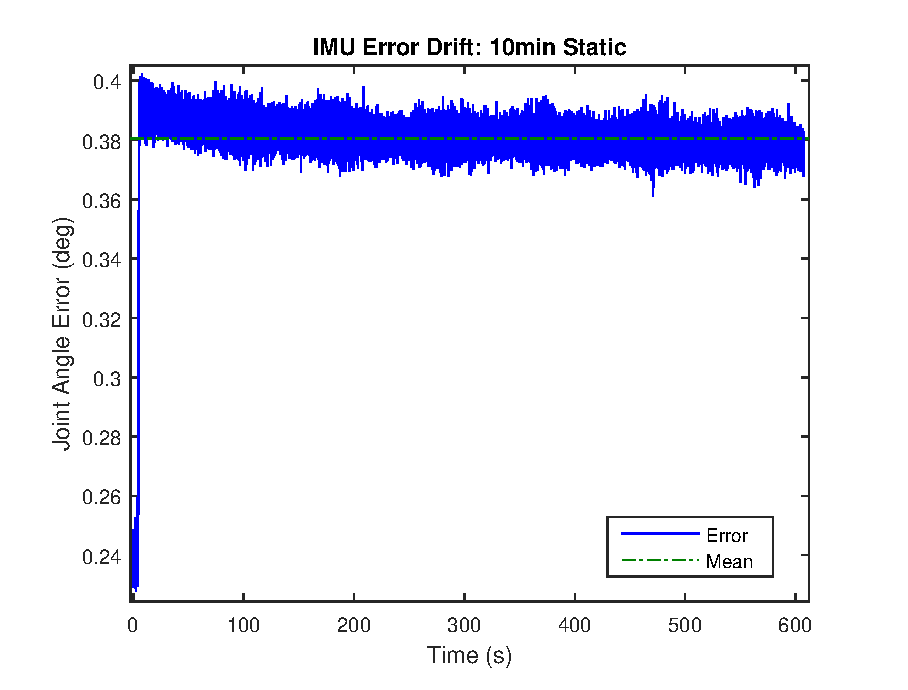
\includegraphics[width = 3.5in]{static_drift.eps}
    \caption{Drift error over time for static test. Mean error: 0.3804\degree}
    \label{fig:staticDrift}
\end{figure}

The drift started at about 0.2 degrees from zero, quickly moved to 0.4 degrees, and remained at about that amount for the remaining time. Some change in error occurred initially, but the IMU reported joint angle appeared to remain fairly accurate an non-changing over the duration of the test. Most importantly, this suggested that the IMU did not experience appreciable drift over longer lengths of time. In addition, because the IMU data resolution was on a scale of about 0.1 degrees, these discrepancies were not far out of specification. This also provided a potential baseline accuracy for examining other tests. 

The finger bending tests were conducted next. The results of the experiment are shown in \autoref{fig:bendPlot0min}, which shows the joint angles just after the start of the experiment.

\begin{figure}[thpb]
	\centering
	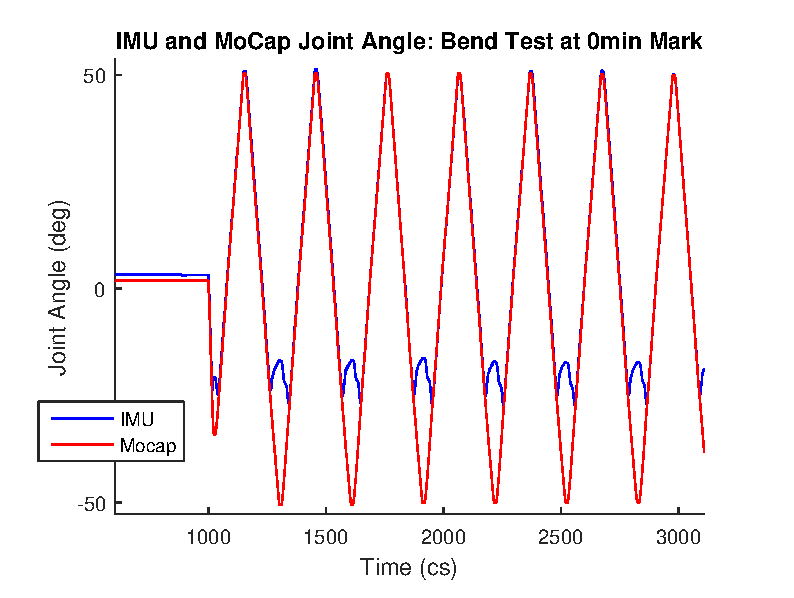
\includegraphics[width = 3.5in]{finger_bend_imuANDmocap_0min.eps}
    \caption{Plot of mocap and IMU joint angles at the start of the bend test.}
    \label{fig:bendPlot0min}
\end{figure}

There was a small non-zero error at the start of the experiment before the bending motion commenced. The IMU reported angle suffered from artifacts at the negative joint angle values, experiencing a defect at around -25\degree. This was caused by a Euler angle wrap around that was not accounted for in the MATLAB results gathering. Unfortunately, it was unable to be fixed in a timely manner. However, even with this artifact, it can be shown that the IMU remained in good accuracy and the time was properly synchronized between the systems. Peaks of positive joint angles were very close in value, within a degree, and stayed consistent for several seconds. 

In order to examine the long-term accuracy of the system, the plot was analyzed again close to the five minute mark in the experiment, shown in \autoref{fig:bendPlot5min}.

\begin{figure}[thpb]
	\centering
	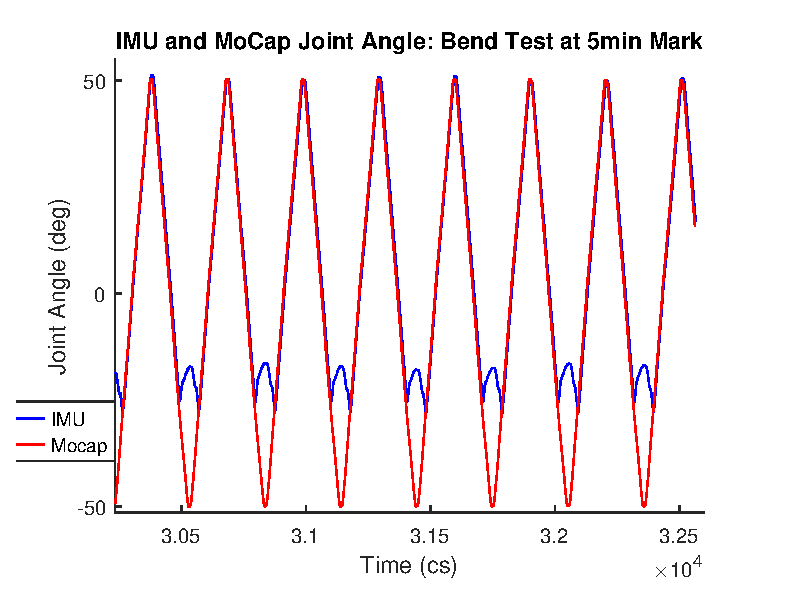
\includegraphics[width = 3.5in]{finger_bend_imuANDmocap.eps}
    \caption{Plot of mocap and IMU joint angles five minutes into bend test.}
    \label{fig:bendPlot5min}
\end{figure}

The same artifact appeared at the same joint angle, but more importantly, there was not a significant change in the angle as reported by both systems. The IMU did accumulate a slight error, as the positive angle peaks were closer to about 1.5-2/degree higher than the mocap data and the rise and fall had a slight latency compared to the plot taken at the start of the test. These results seemed to indicate that prolonged bending motions did not cause errors to accumulate between the mocap and IMU-reported joint angle. While the MATLAB scripts to process the data included a defect with wrapping Euler angles around a 90/degree mark, an implemented system utilizing the quaternion would not see the effect if properly constructed.

\subsection{Motion}
Unfortunately, both the circular and linear motion tests included instances where the mocap system lost tracking of the markers. Due to timing constraints, this data was unable to be cleaned sufficiently to include in the paper. However, the shaking tests, arguably more relevant, worked appropriately and were analyzed below.

Shaking motion was tested to see if rapid changes would impact the accuracy of the joint angle as reported by the IMU. \autoref{fig:shakingDrift} shows the drift error over time while the finger link was shaken as if held by a person suffering from Parkinson's Disease.

\begin{figure}[thpb]
	\centering
	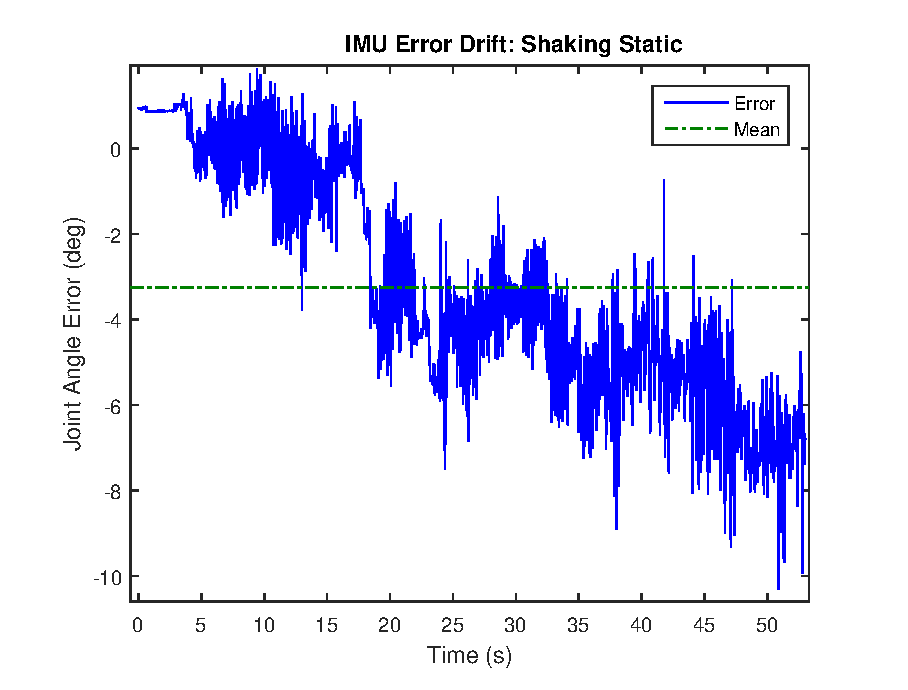
\includegraphics[width = 3.5in]{shaky_static_drift.eps}
    \caption{Drift error over time with violent shaking. Mean error: -3.250\degree}
    \label{fig:shakingDrift}
\end{figure}

Error between the mocap system and the IMU accumulated rapidly in this test. There was an unknown artifact at the beginning of the trial that reported a steady-state error of one degree, but as evidenced by the remainder of the trial, this was fairly insignificant. At worst, the error approached about 10\degree, with an average of 3.25\degree. Depending on the application requirements, this could indicate that an IMU-based solution for tracking finger pose would be insufficient for patients with Parkinson's disease, as shaking accumulates rather noticeable errors over time.

\subsection{Environmental Interference}

Magnetic and ferrous materials with EMF noise were introduced into the testing environment. \autoref{fig:ferrousDrift} shows the IMU drift error over the course of the testing for when the two-link system was kept still.

\begin{figure}[thpb]
	\centering
	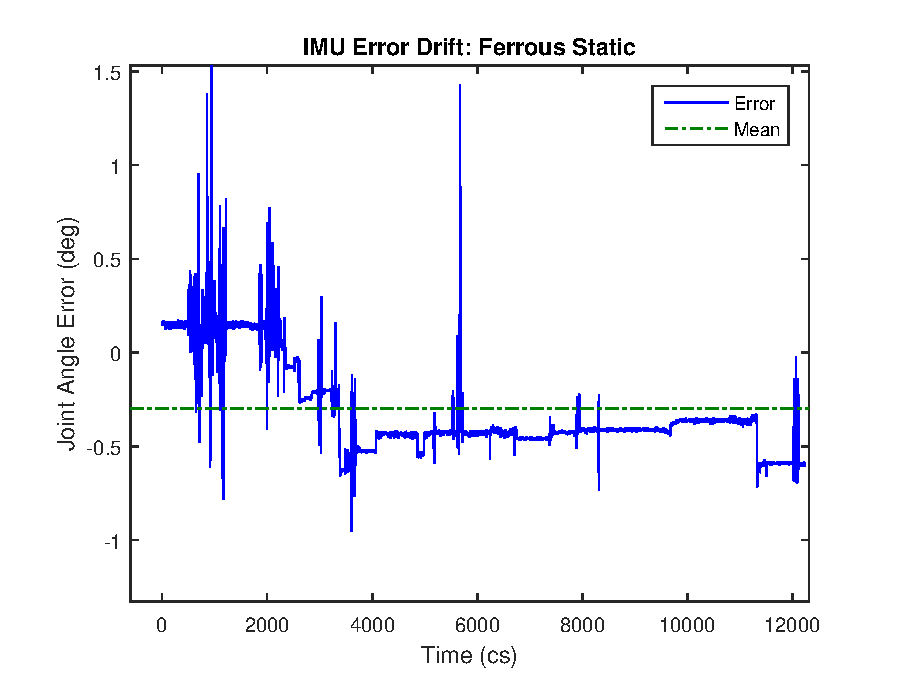
\includegraphics[width = 3.5in]{ferrous_static_drift.eps}
    \caption{Drift error over time with ferrous materials in environment. Mean error: -0.297\degree}
    \label{fig:ferrousDrift}
\end{figure}

It can be seen that the error increased to about half a degree once the materials were introduced and moved around, but the error did not grow significantly during the test. Towards the end of the test, when the cell phone was called and the ferrous material was removded, the error increased again. This indicated that the removal or addition of ferrous materials changed the error of the system, but the error tended to remain fairly steady. It was possible that the phone call had some effect on the system, but this should have been conducted in an independent test. Large spikes in the middle of the data set reflect changes in the mocap reported angle, which could have been due to occlusions.

In another test, magnets were waved around the device as it remained at rest. \autoref{fig:magneticDrift} shows the plot of error over time.
\begin{figure}[thpb]
	\centering
	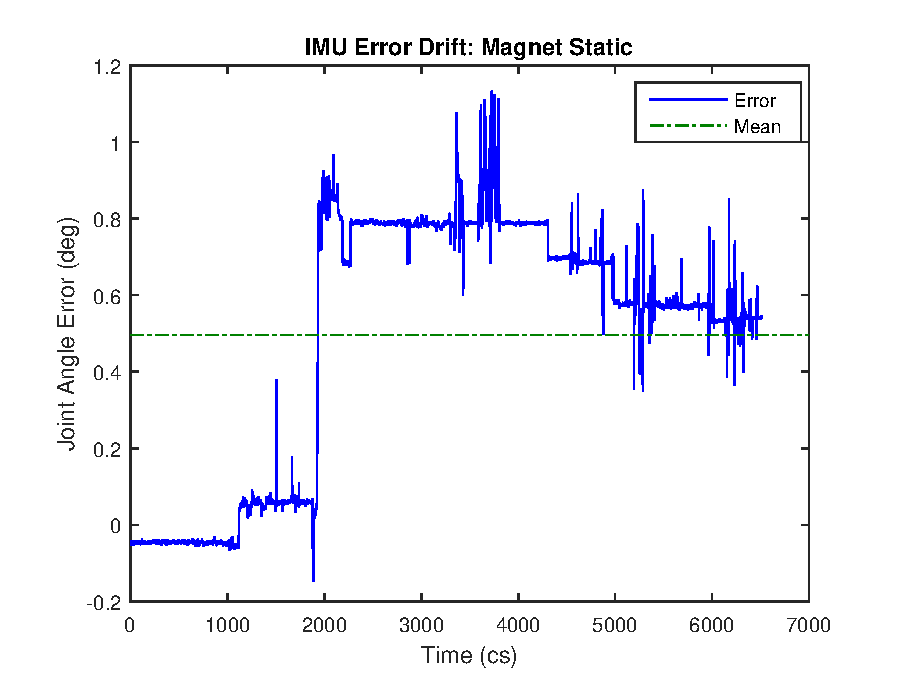
\includegraphics[width = 3.5in]{magnet_static_drift.eps}
    \caption{Drift error over time with magnetic materials in environment. Mean error: 0.496\degree}
    \label{fig:magneticDrift}
\end{figure}

The magnetic disturbance test showed a large, sudden change in error after the magnets began to be introduced. Similar to the ferrous material test, the error did not continue to worsen, but the error also did not tend to return to zero, as in the other test. Rather, it remained about 0.5\degree towards the termination of the test. This would seem to indicate that the active presence of magnets causes greater disturbances than ferrous material. 

%%%%%%%%%%%%%%%%%%%%%%%%%%%%% FUTURE WORK %%%%%%%%%%%%%%%%%%%%%%%%%%%%%%%%%
\section{FUTURE WORK AND RECOMMENDATIONS}

While the finger bending motion was fairly well controlled by the servo, regular motions of the entire system were less consistent. The finger-servo mechanism can be attached to the end of an ABB arm, allowing controlled and repeatable motion of the entire system. This would provide an excellent basis for determining the accuracy of the system as a whole. While the ABB arm contains ferrous materials, results indicate that the errors may be low enough to warrant introducing the ABB arm as the testing device. Further, if the calibration of the IMU's was conducted on the arm itself, the ferrous materials in proximity to the IMU sensor may not have as great an impact.

The ribbon cables connected to the sensors seemed fragile or perhaps too high a gauge. During testing, the two sensors that were wired with the thinner ribbon cable experienced intermittent failure and connection issues. They were swapped with the sensors with the originally equipped ribbon cable, which was of a lower gauge, and the connection errors were significantly reduced. The wires should be investigated to determine if significant voltage drop or breakage was causing issues with the sensor operation.

There are some methods in which the tests conducted could be improved. The first would be to duplicate experiments several times while testing for the same effect. Only having one trial for each variable does not allow sufficiently significant data to draw conclusions. Further, introduction of environmental factors should have been timestamped properly to better view the appropriate change in error. 

Similarly, a rest period could be introduced at the end of the trial to see if error tended towards zero after motions. Calibration motions could also be carried out after the rest period to see if the sensors could properly recover from significant drift accumulation. 

The magnetic tests could have been more severe. Rather than wand around a pack of magnets, the sensors could have been placed between a pair of magnets such that they were completely inside of the magnetic field. This would have demonstrated a better worse-case scenario.

The IMU's themselves should be investigated more thoroughly to determine what types of filter parameters, if any, are easily exposed to the user. This could allow more sophisticated calibration routines. For instance, a calibration can be saved into a particular register and loaded on start-up. This should be tested to see if the timely calibration period at the beginning of each trial can be safely bypassed. Finally, it would be of benefit to test a single IMU unit in examining per-axis drift and error over time. Unfortunately, this project did not have enough time to conduct a more thorough analysis of the IMU as an independent unit.

%%%%%%%%%%%%%%%%%%%%%%%%%%%%% CONCLUSION %%%%%%%%%%%%%%%%%%%%%%%%%%%%%%%%%
\section{CONCLUSION}
This project successfully created a test bed and conducted a series of tests to determine the accuracy of an IMU-based hand pose tracking system. Fixtures were created to automate bending tests with a servo, and Arduino code was modified to allow quaternion orientation capture from both IMU's on an Arduino Mega. An OptiTrack mocap system was successfully used to synchronize data collection and provide ground truth for determining system accuracy. MATLAB scripts were able to calculate the joint angle somewhat accurately and provide error terms over time for the system. 

Testing showed that in static tests the IMU did not accumulate more than 0.4\degree of joint angle error, even after 10 minutes. Finger bending tests, while affected by a Euler angle defect, indicated that the IMU was able to maintain less than 2\degree of error, though typically within 1\degree, after five minutes of continuous bending motions. Shaking motions accrued errors up to 10\degree from truth after a few moments, the worst errors seen during testing. Ferrous material interference introduced stead-state errors of around 0.5\degree, while magnetic interference produced joint angle errors of around 0.8-1\degree. This indicated ferrous and magnetic interference introduce a small but appreciable amount of error over the static baseline test. These tests, while not exhaustive, demonstrated typical IMU-provided joint angle errors in situations that could be encountered during stroke patient rehabilitation and Parkinson's Disease research when utilizing an IMU-based hand pose tracking system. 

\addtolength{\textheight}{-12cm}   % This command serves to balance the column lengths
                                  % on the last page of the document manually. It shortens
                                  % the textheight of the last page by a suitable amount.
                                  % This command does not take effect until the next page
                                  % so it should come on the page before the last. Make
                                  % sure that you do not shorten the textheight too much.

%%%%%%%%%%%%%%%%%%%%%%%%%%%%% APPENDIX %%%%%%%%%%%%%%%%%%%%%%%%%%%%%%%%%
\section*{APPENDIX}
The Arduino and MATLAB source code for this project can be found at our GitHub repository:  \href{https://github.com/ChrisBove/HandPoseTracking}{ChrisBove/HandPoseTracking}.
The final presentation can be viewed on \href{https://docs.google.com/presentation/d/1VDLMp_ZAbCT3yII7-D-Xm1Q3-hwkLWy0UZxRYme4dzw/edit?usp=sharing}{Google Drive}.

\section*{ACKNOWLEDGMENT}
Our team would like to thank our adviser Professor Gregory Fischer for his guidance and assistance during this project. We also thank Chris Nycz, WPI AIM Lab, for his assistance setting up the OptiTrack hardware and interfacing with the IMU sensors.  

%%%%%%%%%%%%%%%%%%%%%%%%%%%%% BIBLIOGRAPHY %%%%%%%%%%%%%%%%%%%%%%%%%%%%%%%%%
\begin{thebibliography}{99}

\bibitem{Patel} Patel, S., Park, H., Bonato, P., Chan, L., and Rodgers, M. (2012). A review of wearable sensors and systems with application in rehabilitation. Journal of NeuroEngineering and Rehabilitation J NeuroEngineering Rehabil, 9(1), 21. doi:10.1186/1743-0003-9-21
\bibitem{Perumal} Perumal, S. V., and Sankar, R. (2016). Gait and tremor assessment for patients with Parkinson’s disease using wearable sensors. ICT Express. doi:10.1016/j.icte.2016.10.005
\bibitem{Sokal} Sokal, B., Uswatte, G., Barman, J., Brewer, M., Byrom, E., Latten, J., . . . Sarkar, N. (2014). Network of Movement and Proximity Sensors for Monitoring Upper-Extremity Motor Activity After Stroke: Proof of Principle. Archives of Physical Medicine and Rehabilitation, 95(3), 499-505. doi:10.1016/j.apmr.2013.09.013
\bibitem{Zhou} Zhou, H., and Hu, H. (2008). Human motion tracking for rehabilitation—A survey. Biomedical Signal Processing and Control, 3(1), 1-18. doi:10.1016/j.bspc.2007.09.001 

\end{thebibliography}

\end{document}
